\documentclass[11pt]{article}
\usepackage[a4paper,margin=2.6cm]{geometry}
\usepackage[T1]{fontenc}
\usepackage[utf8]{inputenc}
\usepackage{times}
\usepackage{microtype}
\usepackage{booktabs}
\usepackage{graphicx}
\usepackage{amsmath}
\usepackage[numbers,sort&compress]{natbib}
\usepackage[hidelinks]{hyperref}
\usepackage{caption}
\usepackage{enumitem}
\captionsetup{font=small,labelfont=bf}
\setlist{nosep}

\title{The Direction of a Dependency-Length Comparison Depends on How Hard the Baseline Is}
\author{Bart{\l}omiej Nawara\\Independent researcher, Poland\\\texttt{barteknawara@gmail.com}}
\date{November 2026}

\begin{document}
\maketitle

\begin{abstract}
Dependency length minimization (DLM) is usually shown by comparing attested word orders with random relinearizations of the same trees. That comparison needs two choices that are rarely reported together: the baseline the attested order is measured against, and the effect measure that summarises the comparison. We show that the answer depends on them. Testing the claim of \citet{yadav2022reappraisal} that the number of intervening syntactic heads, rather than the number of intervening words, is the quantity languages minimise, we find that rank-based and magnitude-based effect measures disagree about which metric shows the larger effect in 26 of 26 Universal Dependencies treebanks under a uniform random baseline, and in 6 of 26 under a stricter arity-preserving one. Because those two baselines differ in more than difficulty, we build a baseline of tunable difficulty that interpolates between the uniform baseline and the attested order, and sweep it. The disagreement grows monotonically as the baseline becomes easier to beat (9 of 9 steps; $r=-0.96$ between the interpolation parameter and the divergence), the trend holds in each of the 26 treebanks, and it survives treating language family rather than treebank as the unit (mixed model slope $-0.24$, 95\% CI $-0.28$ to $-0.20$). We also report two statistics that produce their own results: a shrinkage criterion across nested logistic models, which fails in both directions because logistic coefficients are not collapsible, and a rank measure pre-registered as tie-immune, which equals $(1-\delta)/2$ identically. The narrow conclusion is that the comparative claim holds on a magnitude reading and fails on a rank reading. The general one is that the direction of a DLM comparison computed against one baseline with one effect measure is a function of a design choice.
\end{abstract}

\section{Introduction}

Dependency length minimization is among the most cited quantitative regularities in linguistics. Across languages, attested word orders keep heads and their dependents closer together than chance arrangements of the same trees would \citep{ferrericancho2004euclidean,liu2008dependency,gildea2010grammars,futrell2015largescale,temperley2018minimizing}.

The standard measure counts \emph{words} between head and dependent. \citet{yadav2020wordorder} introduced intervener complexity, the number of syntactic \emph{heads} between them, and \citet{yadav2022reappraisal} argue that it captures the cross-linguistic pattern better than word-based length and that minimising it is a constraint in its own right. If so, much of the corpus literature has been measuring a correlate of the quantity that matters.

The claim is cheap to test. Both measures come off the same trees, so no new annotation is needed, only a decision about what to compare them against, and how. This paper is about those decisions. We set out to test the claim and could not answer it without first answering a prior question: how much of a DLM comparison is fixed by its own design? Enough to reverse it.

\paragraph{What we claim.}
\begin{enumerate}
  \item Rank-based and magnitude-based effect measures disagree systematically about the word-versus-head comparison, and the disagreement is controlled by baseline difficulty rather than by any property of the two metrics.
  \item This is shown by a controlled sweep, not inferred from contrasting two fixed baselines, and it holds within every language family in the sample.
  \item Two reasonable-looking statistics, a nested-model shrinkage criterion and a tie-splitting rank measure, produce results without corresponding facts. We characterise both failures.
\end{enumerate}

\paragraph{What we do not claim.} We do not settle whether head-based dependency length is the better construct. Our results are consistent with head-based length showing the larger effect on a magnitude reading under both baselines and the smaller one on a rank reading, and nothing in corpus data alone decides which reading is right.

\section{Related work}
\label{sec:related}

\paragraph{DLM and its baselines.} \citet{ferrericancho2004euclidean} compared observed dependency distances with random linear arrangements of the same sentences, and \citet{liu2008dependency} reported mean dependency distance for twenty languages against two random baselines. \citet{gildea2010grammars} compared attested orders with random and with optimal projective orders of the same trees and found English and German closer to the optimum than to chance. \citet{futrell2015largescale} extended the comparison to 37 languages and made the choice of baseline explicit: free random projective orders, and random orders that fix each head's direction, with the effect visible against both. \citet{temperley2018minimizing} and \citet{futrell2020locality} review the evidence and its interpretation. \citet{ferrericancho2022optimality} define a score that places observed sums of distances between the random-baseline expectation and the minimum, which makes the dependence on the baseline part of the quantity itself. Our contribution is narrower and methodological: holding trees fixed and varying only the difficulty of the baseline, we show that the \emph{direction} of a comparison between two length metrics, not only its size, depends on that choice.

\paragraph{Intervening heads.} \citet{yadav2020wordorder} proposed counting intervening heads and found it to interact with word-order typology; \citet{yadav2022reappraisal} argue that intervener complexity is minimised beyond what word-based length explains. Recent work on functional versus lexical relations \citep{gerdes2026grammar} also finds that what looks like a single minimisation pressure decomposes along the annotation scheme's choices of headedness, a theme that returns in our limitations: the count of intervening heads is defined by those choices.

\paragraph{Effect measures and nested models.} Cliff's $\delta$ \citep{cliff1993dominance} is the rank measure used throughout. The failure in Section~\ref{sec:shrinkage} is an instance of a known property: coefficients in logistic regression change when a predictor carrying real signal is added, even without confounding, so comparisons of coefficients across nested logit models do not measure mediation \citep{mood2010logistic}. We control the false discovery rate across treebanks within each hypothesis family \citep{benjamini1995fdr}.

\section{Setup}
\label{sec:setup}

\paragraph{Data.} Universal Dependencies v2.14 \citep{zeman2024ud214}, training splits. Of 29 configured treebanks, 26 cleared a 1,500-sentence floor after validation (Table~\ref{tab:treebanks}). Sentences are filtered to 3--100 tokens and multiword tokens and empty nodes are dropped, which leaves 480,515 sentences; the 430,113 projective ones (7,118,952 arcs) enter the analysis. The sample is typologically uneven: 15 of 26 treebanks are Indo-European, Afro-Asiatic, Uralic and Turkic have two each, and Japonic, Koreanic, Sino-Tibetan, Austronesian and Basque one each. Section~\ref{sec:family} tests whether that matters. Licences differ by treebank: 14 of the 26 are released under CC~BY or CC~BY-SA and 12 under CC~BY-NC-SA (Table~\ref{tab:treebanks}). The repository redistributes no treebank text, only per-treebank aggregate statistics.

\paragraph{Metrics.} For a sentence with arcs $(h,d)$, \emph{word\_DL} is $\sum |h-d|$ and \emph{head\_DL} is $\sum$ (number of syntactic heads strictly between $h$ and $d$). A vectorised head-counting path was checked against a naive $O(n^2)$ reference on every valid tree with $n\le 7$, in both scope settings, with no mismatches.

\paragraph{Baselines.} Each real sentence is paired with random projective relinearizations of its own tree, so tree shape is held fixed by construction. \textbf{B1 (uniform)}: at each node the head and its subtree blocks are shuffled uniformly. \textbf{B2 (arity-preserving)}: the shuffle keeps each node's numbers of left and right dependents, so branching direction is fixed. Twenty relinearizations per sentence are averaged, giving one matched baseline value per sentence and metric. Non-projective sentences are excluded and counted separately, since a projective baseline is not comparable to a non-projective original; all results are conditional on projectivity.

\paragraph{Effect measures.} Three summaries of the same paired comparison: Cliff's $\delta=(\#\text{real}>\text{base}-\#\text{real}<\text{base})/n$ (rank); $P(\text{adv})=(\#\text{real}<\text{base}+\tfrac12\#\text{ties})/n$ (rank); and the median of $(\text{base}-\text{real})/\text{base}$ (magnitude). The quantity of interest is the contrast between metrics, e.g.\ $\Delta|\delta| = |\delta_{\text{head}}|-|\delta_{\text{word}}|$, positive when it favours head\_DL. Confidence intervals use a paired bootstrap that draws one set of sentence indices per replicate and applies it to all four arrays, which keeps the correlation between metrics.

\paragraph{Pre-registration and deviations.} Decision rules were written to \texttt{config.yaml} before results were generated, and \texttt{verdict.json} echoes them back, with a test asserting the two match. A hypothesis is \textsc{supported} if at least 70\% of conditions show the predicted effect with a 95\% CI excluding zero, \textsc{contradicted} below 30\%, \textsc{equivocal} otherwise. A condition is a treebank for the sanity check and a treebank $\times$ baseline cell for the comparative hypotheses. Two deviations are recorded rather than hidden. (i) The pre-registered H3 criterion, at least 50\% shrinkage of $|\beta(\text{word\_DL})|$ when head\_DL is added, was retired after we found it invalid (Section~\ref{sec:shrinkage}); \texttt{config.yaml} keeps it as an explicit null with the reason, and a test asserts it stays retired. H3 is scored instead on a conditional logit with a nested likelihood-ratio test, which was not pre-registered. (ii) An earlier write-up cited validation numbers for three treebanks that no code in the repository produced. Recomputation matched two and missed the third by 0.14 in $\delta$; those numbers were withdrawn, and \texttt{verify\_finding1.py} recomputes the replacements. The $\lambda$-sweep of Section~\ref{sec:sweep} and the family analysis of Section~\ref{sec:family} were added after the main run.

\section{The comparison disagrees with itself}
\label{sec:h2}

DLM replicates as a sanity check: real orders are shorter than random projective relinearizations on both metrics in 26 of 26 treebanks, all CIs excluding zero. Japanese is strongest ($\delta_{\text{word}}=-0.971$), German weakest ($-0.412$), in line with their branching rigidity. The comparative question gets three answers depending on the statistic:

\begin{center}\small
\begin{tabular}{lllr}
\toprule
statistic & kind & verdict & cells \\
\midrule
$\Delta|\delta|$ & rank & \textsc{contradicted} & 12/52 \\
$\Delta P(\text{adv})$ & rank & \textsc{equivocal} & 17/52 \\
$\Delta$ median rel.\ reduction & magnitude & \textsc{supported} & 44/52 \\
\bottomrule
\end{tabular}
\end{center}

Under B1 the split is total. The magnitude measure favours head\_DL in 26/26 treebanks and the rank measures favour word\_DL in 26/26; no treebank goes the other way on either. Both readings describe something real. By rank, word\_DL wins: median $P(\text{real shorter})$ is 0.861 for word\_DL against 0.783 for head\_DL. By magnitude, head\_DL wins: median per-sentence reduction is 0.325 against 0.190, so when head\_DL separates attested from random it does so by about 1.7 times the proportional margin. head\_DL wins fewer pairs and wins them by more. Under B2 the rank and magnitude measures point in opposite directions in only 6 of 26 treebanks; rank favours head\_DL in 12/26 and magnitude in 18/26.

\section{Baseline difficulty, controlled}
\label{sec:sweep}

Section~\ref{sec:h2} is suggestive but correlational. B1 and B2 differ in more than difficulty, since B2 also fixes branching direction, so their contrast cannot separate ``difficulty causes the divergence'' from ``branching does''.

\paragraph{A baseline of tunable difficulty.} At every node independently, the attested local arrangement is kept with probability $\lambda$ and replaced by a uniform shuffle otherwise. $\lambda=0$ is B1 and $\lambda=1$ is the attested sentence, with the construction fixed throughout. Interpolating per node rather than per sentence matters: mixing whole sentences gives a bimodal mixture of attested and fully scrambled items, whose rank statistic averages two extremes instead of reaching an intermediate difficulty. Tests assert both endpoints ($\lambda=0$ reproduces B1 sample for sample; $\lambda=1$ is an exact identity on projective sentences), preservation of the arc multiset, and monotonicity of mean word\_DL in $\lambda$.

\paragraph{Why interpolate towards the attested order.} The family is not a claim about which baseline is right; it is the cheapest one-parameter family that changes difficulty while holding everything else fixed. Any harder baseline built by a different mechanism, B2 included, changes difficulty together with some structural property of the orders it admits, and that is the confound the sweep exists to remove. Interpolating towards the attested order has one cost: at high $\lambda$ the baseline inherits language-specific structure, so between-language comparisons at a given $\lambda$ are not comparisons at equal difficulty. We therefore make within-language statements (each treebank centred on its own mean) and read the pooled numbers as summaries.

\paragraph{Predictions,} stated in the script before it ran. P1: rank separation between metrics shrinks towards zero as $P(\text{adv})$ approaches its ceiling. P2: magnitude separation does not shrink the same way. P3: the two diverge monotonically, so the sign flip is a property of difficulty rather than of B1's construction.

\begin{figure}[t]
\centering
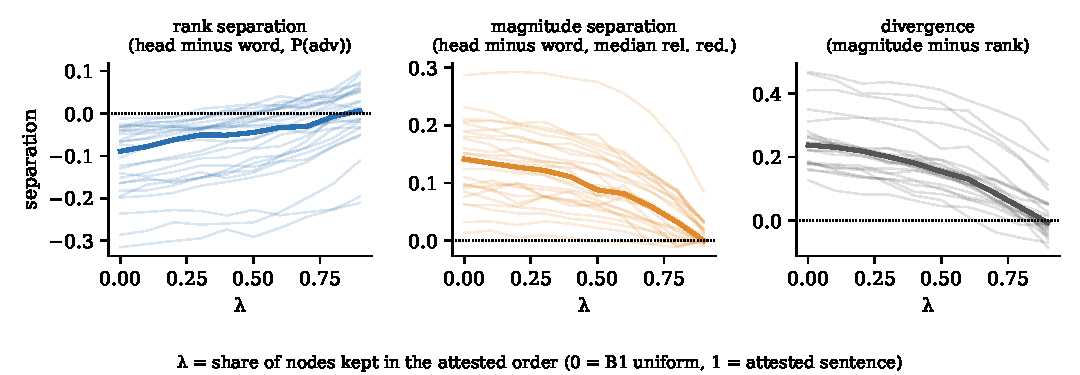
\includegraphics[width=\linewidth]{figs/fig_d_lambda_sweep.pdf}
\caption{Rank separation ($\Delta P(\text{adv})$), magnitude separation ($\Delta$ median relative reduction) and their divergence across the $\lambda$ sweep. Thin lines: the 26 treebanks; thick lines: median across treebanks. Positive values favour head\_DL.}
\label{fig:sweep}
\end{figure}

\paragraph{Result.} Sweeping $\lambda$ over ten values on all 26 treebanks (Figure~\ref{fig:sweep}):

\begin{center}\small
\begin{tabular}{rrrrr}
\toprule
$\lambda$ & $P(\text{adv})$, best metric & rank sep. & magnitude sep. & divergence \\
\midrule
0.0 & 0.817 & $-0.114$ & $+0.137$ & 0.251 \\
0.2 & 0.807 & $-0.098$ & $+0.127$ & 0.226 \\
0.4 & 0.791 & $-0.081$ & $+0.114$ & 0.196 \\
0.6 & 0.765 & $-0.059$ & $+0.089$ & 0.148 \\
0.8 & 0.714 & $-0.025$ & $+0.041$ & 0.066 \\
0.9 & 0.664 & $-0.002$ & $+0.013$ & 0.015 \\
\bottomrule
\end{tabular}
\end{center}

The divergence rises on 9 of 9 steps as the baseline gets easier, with $r(\lambda,\text{divergence})=-0.964$, and there are no exceptions across treebanks: $r(\lambda,\text{rank sep.})>0$ in 26/26 (median $+0.96$, minimum $+0.49$), $r(\lambda,\text{magnitude sep.})<0$ in 26/26 (median $-0.94$, maximum $-0.84$), and the divergence is monotone ($r<-0.8$) in 26/26.

P3 held: the B1-versus-B2 contrast was not a quirk of B2's construction, and difficulty alone reproduces the effect. P1 as written was wrong, and we report the failure rather than substituting a corrected test. By the literal prediction $|\text{rank sep.}|$ does not shrink (0.106 easy against 0.059 hard). Two things were wrong with the formulation. Rank separation is signed, so its absolute value hides the pattern: against an easy baseline the rank statistic says word\_DL wins by a lot, and that advantage decays towards zero as the baseline hardens. And pooling across treebanks destroys the ceiling correlation, $r=-0.16$ pooled against $-0.90$ once each treebank is centred on its own mean; baseline difficulty is comparable within a language but confounded with branching profile between languages. P2 held, but not as assumed: difficulty does not saturate one measure and spare the other, it drives both, in opposite directions.

\paragraph{Interpretation.} A rank statistic asks how often the attested order wins. Against an easy baseline it wins almost always on both metrics, so the statistic approaches its ceiling and loses the resolution to separate them. A magnitude statistic asks by how much, and keeps resolution there. As the baseline hardens the rank statistic regains discrimination while the magnitude gap narrows, and the two converge.

\subsection{Language family as the unit}
\label{sec:family}

``26 of 26 treebanks'' counts Indo-European fifteen times. We therefore repeated the sweep analysis with family as the unit (\texttt{experiment\_family\_sensitivity.py}, added after the main analysis). The within-treebank-centred correlation between $\lambda$ and the divergence is negative in every one of the nine families, from $-0.82$ (Japonic, one treebank) to $-0.98$ (Sino-Tibetan); it is $-0.94$ within Indo-European and $-0.91$ across the eleven treebanks outside it. Dropping any one family leaves the pooled centred correlation between $-0.931$ and $-0.908$ (Table~\ref{tab:family}). A mixed model with random intercepts and $\lambda$ slopes by family and a variance component for treebank within family gives a fixed $\lambda$ slope of $-0.238$ (95\% CI $-0.276$ to $-0.199$), and a cluster bootstrap that resamples families gives $-0.268$ to $-0.207$ for the pooled within-treebank slope, negative in all 5,000 resamples. Six of the nine families are represented by a single treebank, so this establishes that no family drives or reverses the trend, not that the trend is typologically universal.

\begin{table}[t]
\centering\small
\caption{Robustness of the $\lambda$-sweep result by language family. $r$ and slope: within-treebank-centred correlation and slope of the divergence on $\lambda$ inside the family. Last column: pooled centred $r$ over all treebanks with that family removed (all treebanks: $-0.926$). Source: \texttt{results/family\_sensitivity.json}.}
\label{tab:family}
\begin{tabular}{lrrrr}
\toprule
family & treebanks & $r$ & slope & $r$ without family \\
\midrule
Indo-European & 15 & -0.94 & -0.26 & -0.908 \\
Afro-Asiatic & 2 & -0.91 & -0.17 & -0.931 \\
Turkic & 2 & -0.93 & -0.30 & -0.927 \\
Uralic & 2 & -0.97 & -0.28 & -0.922 \\
Austronesian & 1 & -0.95 & -0.20 & -0.926 \\
Japonic & 1 & -0.82 & -0.20 & -0.930 \\
Koreanic & 1 & -0.92 & -0.23 & -0.926 \\
Sino-Tibetan & 1 & -0.98 & -0.15 & -0.928 \\
isolate & 1 & -0.96 & -0.33 & -0.926 \\
\bottomrule
\end{tabular}

\end{table}

\section{Two statistics that produce their own results}

\subsection{Shrinkage across nested logistic models}
\label{sec:shrinkage}

The natural test of ``word\_DL is derivative of head\_DL'' is whether word\_DL's coefficient collapses once head\_DL is controlled, and we pre-registered a 50\% shrinkage criterion on $|\beta(\text{word\_DL})|$ across nested models. The criterion is invalid: logistic coefficients are not collapsible \citep{mood2010logistic}, so adding a predictor that carries real signal rescales the others even when nothing is confounded. Simulation with known ground truth shows the statistic failing in both directions. With independent causes, where derivativeness is false, it reports up to $+73\%$ shrinkage. With a head-only cause and word\_DL's true effect exactly zero, where derivativeness is true, it reports $-81\%$, which reads as ``suppression''. An earlier version of our own write-up interpreted negative-shrinkage cells as suppression; they were this artefact.

A second defect compounded it. The model was a plain logistic regression with \texttt{n\_tokens}, \texttt{mean\_arity} and \texttt{tree\_depth} as covariates. Because the design is matched pairs, all three are constant within a pair and control nothing; the pairing does that work. The right model is a conditional logit stratified on the pair, where such covariates drop out by construction.

Rescored on the conditional logit, with a nested likelihood-ratio test under FDR control and within-pair $\Delta$AUC, derivativeness is contradicted: $\beta(\text{word\_DL})$ stays significant in 50 of 52 cells once head\_DL is controlled (median $-8.74$ against $-0.17$ for head\_DL), and adding word\_DL to head\_DL improves within-pair discrimination by $\Delta\text{AUC}=+0.036$. Two caveats. Within pairs the two metrics' differences correlate at 0.95--0.98 (VIF up to 41), so individual coefficients are jointly identified but individually fragile; the AUC gain and the LR test are the interpretable quantities. And $\beta(\text{head\_DL})$ has the wrong sign in 25 of 52 cells across 18 of the 26 languages, concentrated under B1 (18/26 against 7/26 under B2), which points back to the difficulty mechanism of Section~\ref{sec:sweep} rather than to a linguistic fact.

\subsection{A tie-splitting rank measure that is not a new measure}

head\_DL is much coarser than word\_DL and ties with its baseline far more often (median 4.25\% against 0.21\% under B1). Since Cliff's $\delta$ appears to count every tie as non-support, we pre-registered $P(\text{adv})$ with ties split evenly as a tie-immune co-primary. The premise was wrong. With $pos+neg+ties=n$,
\[
\delta=\frac{pos-neg}{n},\qquad P(\text{adv})=\frac{neg+ties/2}{n}=\frac{1-\delta}{2}\quad\text{exactly, ties included.}
\]
$\delta$ already splits ties: a tie contributes to neither $pos$ nor $neg$, which is arithmetically the same as contributing half to each. Across all 52 cells $r(\Delta P(\text{adv}),\Delta\delta)=1.0$ at a ratio of exactly 0.5. The pre-registered design bought one contrast, not two. What it delivered was a rank-versus-magnitude contrast, which is the one that carried the result in Section~\ref{sec:sweep}. Pre-registering a statistic does not make it independent of the one it is meant to check; that has to be verified algebraically first.

\section{What this means for DLM work}

The narrow finding: the comparative claim of \citet{yadav2022reappraisal} holds on a magnitude reading (head\_DL shows the larger effect in 26/26 treebanks under B1 and 18/26 under B2) and fails on a rank reading. Corpus data cannot adjudicate between the readings, because they answer different questions: how often, and by how much. The general finding is that a DLM comparison needs a baseline and an effect measure, and the pairing of the two can fix the direction of the result. More data does not fix it: the divergence of Section~\ref{sec:sweep} is monotone and present in every language and every family at more than 400,000 sentences. Three recommendations follow.
\begin{enumerate}
  \item Report both a rank and a magnitude effect measure. They answer different questions and can disagree completely.
  \item Report baseline difficulty explicitly, for example as $P(\text{attested shorter})$. A baseline beaten in 86\% of pairs is near a ceiling, where rank statistics behave badly.
  \item Do not compare coefficients across nested logistic models. Use a likelihood-ratio test or a discrimination measure.
\end{enumerate}

\section{Limitations}

\textbf{Typological coverage.} 15 of 26 treebanks are Indo-European and six of the nine families have one treebank. Section~\ref{sec:family} shows that no family drives the trend; it cannot show that the trend holds for families we did not sample. \textbf{Conditioned on projectivity.} Non-projective sentences (2.5\% of English, 12.3\% of Czech) are excluded, and non-projectivity is plausibly where the two metrics diverge most. \textbf{$\lambda$ interpolates towards the attested order}, not towards a principled notion of a harder baseline. It shows that difficulty drives the divergence; it does not say which difficulty a study should use. \textbf{Annotation conventions are load-bearing.} UD's choices of function-word headedness determine what counts as an intervening head, the exact quantity under test \citep[cf.][]{gerdes2026grammar}. Per-treebank reporting limits but does not remove this, and a replication on SUD-style annotation is the obvious next check. \textbf{Collinearity limits H3.} At VIF up to 41, a null LR result would be hard to tell from lack of power. \textbf{Correlational, not causal.} UD is observational; the findings concern what distinguishes attested orders from random ones, not what speakers do.

\section*{Reproducibility}

{\sloppy
All numbers come from the repository \citep{nawara2026dlm} under a fixed seed (20260919). \texttt{main.py} runs the full analysis (26 treebanks, about 67 minutes); \texttt{verify\_h2\_split.py} recomputes the baseline-dependence table of Section~\ref{sec:h2}; \texttt{experiment\_ceiling.py} runs the $\lambda$ sweep; \texttt{experiment\_family\_sensitivity.py}, \texttt{plot\_sweep.py} and \texttt{paper/make\_tables.py} produce Section~\ref{sec:family}, Figure~\ref{fig:sweep} and the tables from committed results in seconds. \texttt{fetch\_licences.py} records each treebank's licence from its v2.14 README. The test suite (no network) pins the contracts that matter: exact $\lambda$ endpoints, preservation of the arc multiset, agreement of the conditional logit with an independent difference-logit formulation, the retired shrinkage criterion staying retired, and $P(\text{adv})=(1-\delta)/2$. Code is MIT-licensed; treebank licences are as in Table~\ref{tab:treebanks}.\par}

\bibliographystyle{plainnat}
\bibliography{refs}

\appendix
\section{Treebanks}

\begin{table}[h]
\centering\small
\caption{The 26 analysed treebanks (UD v2.14, training splits): family, projective sentences analysed after the 3--100 token filter, share of non-projective sentences excluded, and licence as stated in the treebank's README at tag r2.14 (\texttt{results/treebank\_licences.csv}). hu\_szeged, ta\_ttb and wo\_wtb were configured but fell below the 1,500-sentence floor.}
\label{tab:treebanks}
\begin{tabular}{llrrl}
\toprule
treebank & family & sentences & non-proj.\ \% & licence \\
\midrule
en\_ewt & Indo-European & 11,108 & 2.5 & CC BY-SA 4.0 \\
de\_gsd & Indo-European & 12,480 & 9.5 & CC BY-SA 4.0 \\
fr\_gsd & Indo-European & 13,806 & 4.4 & CC BY-SA 4.0 \\
es\_ancora & Indo-European & 13,417 & 5.7 & CC BY 4.0 \\
ru\_syntagrus & Indo-European & 64,312 & 6.8 & CC BY-NC-SA 4.0 \\
pl\_pdb & Indo-European & 16,789 & 5.1 & CC BY-NC-SA 4.0 \\
cs\_pdt & Indo-European & 144,258 & 12.3 & CC BY-NC-SA 4.0 \\
it\_isdt & Indo-European & 12,683 & 1.3 & CC BY-NC-SA 3.0 \\
pt\_bosque & Indo-European & 6,244 & 8.9 & CC BY-SA 4.0 \\
hi\_hdtb & Indo-European & 11,443 & 14.0 & CC BY-NC-SA 4.0 \\
fa\_seraji & Indo-European & 4,384 & 8.0 & CC BY-SA 4.0 \\
el\_gdt & Indo-European & 1,449 & 11.1 & CC BY-NC-SA 3.0 \\
la\_ittb & Indo-European & 13,221 & 38.3 & CC BY-NC-SA 3.0 \\
ga\_idt & Indo-European & 3,368 & 15.4 & CC BY-SA 3.0 \\
lv\_lvtb & Indo-European & 13,854 & 6.6 & CC BY-SA 4.0 \\
fi\_tdt & Uralic & 11,163 & 6.0 & CC BY-SA 4.0 \\
et\_edt & Uralic & 23,095 & 3.8 & CC BY-NC-SA 4.0 \\
tr\_imst & Turkic & 3,212 & 5.1 & CC BY-NC-SA 4.0 \\
ug\_udt & Turkic & 1,541 & 6.9 & CC BY-SA 4.0 \\
ar\_padt & Afro-Asiatic & 5,321 & 8.4 & CC BY-NC-SA 3.0 \\
he\_htb & Afro-Asiatic & 5,073 & 1.4 & CC BY-NC-SA 4.0 \\
zh\_gsd & Sino-Tibetan & 3,867 & 3.2 & CC BY-SA 4.0 \\
ja\_gsd & Japonic & 6,997 & 0.5 & CC BY-SA 4.0 \\
ko\_kaist & Koreanic & 17,923 & 22.0 & CC BY-SA 4.0 \\
id\_gsd & Austronesian & 4,370 & 2.0 & CC BY-SA 4.0 \\
eu\_bdt & isolate & 4,735 & 12.2 & CC BY-NC-SA 3.0 \\
\midrule
total (26 treebanks) & & 430,113 & & \\
\bottomrule
\end{tabular}

\end{table}

\end{document}
